\begin{frame}
\frametitle{Standards}

		\begin{itemize}
			\item International Telecommunications Union (ITU)
		
			\item Internet Engineering Task Force (IETF)

			\item Commercial entitys
		\end{itemize}

\end{frame}


\begin{frame}
\frametitle{H.323}

	\textbf{Packet-based multimedia communications systems}
	\newline
	\begin{itemize}		
		\item Rigorously defined
		\item Centralised
		\item Designed to fit into existing telco framework
	\end{itemize}

\end{frame}

\begin{frame}
\frametitle{H.323}

	\begin{center} 
  		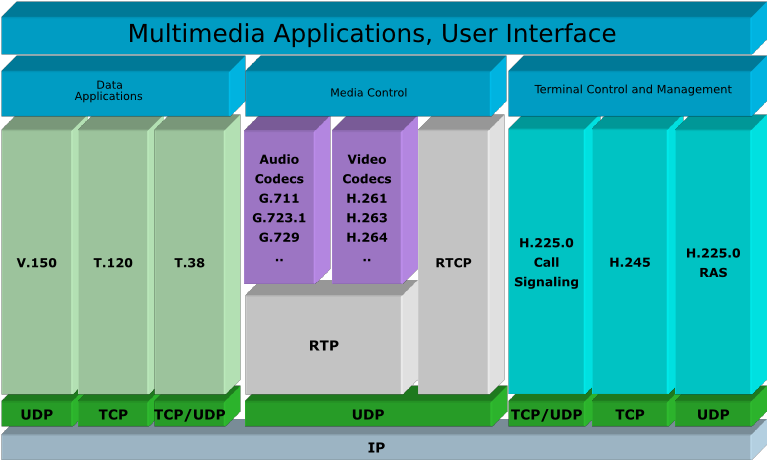
\includegraphics[width=0.9\textwidth]{h323_protocol_overview.png} 
	\end{center} 

\end{frame}

\begin{frame}
\frametitle{SIP}
\textbf{Application-level protocol for inviting users to multimedia conferences}
	\newline
	\begin{itemize}		
		\item Designed with existing internet protocols in mind
		\item Peer-to-peer
		\item Not so strictly defined
	\end{itemize}

\end{frame}


\begin{frame}
\frametitle{Skype}

\begin{itemize}		
		\item Closed source propriety protocol, but due to much research we understand the key elements 
		\item Peer-to-peer with Supern nodes
		\item Voice, video, data and text
	\end{itemize}


\end{frame}


\begin{frame}
\frametitle{Skype}

\begin{center} 
  		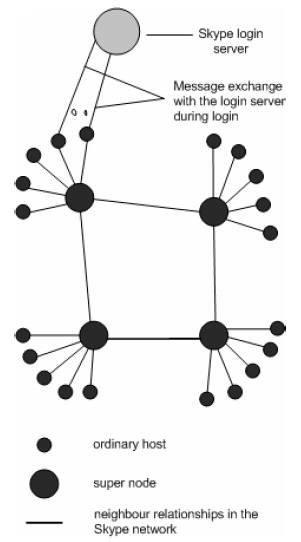
\includegraphics[height=0.9\textheight]{Skype_network2.png} 
	\end{center} 
\end{frame}
